\documentclass[tikz, border=10pt]{standalone}
\usepackage{tikz}
\begin{document}
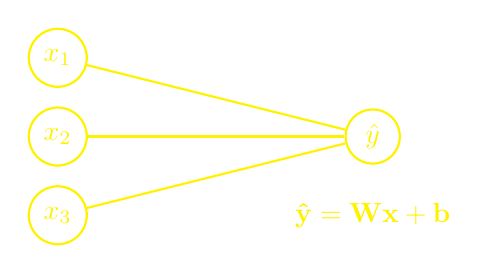
\begin{tikzpicture}[shorten >=0pt, draw=yellow, thick, every node/.style={text=yellow} ] 
    \tikzstyle{neuron}=[circle, minimum size=12pt, draw=yellow, thick, fill=none]  % Circles with yellow boundary
    \tikzstyle{input neuron}=[neuron];
    \tikzstyle{hidden neuron}=[neuron];
    \tikzstyle{output neuron}=[neuron];
    \tikzstyle{annot} = [text width=4em, text centered]

    % Input layer
    \foreach \x in {1,2,3}
        \node[input neuron] (I-\x) at (0,-\x) {$x_\x$};


    % Output layer
    \node[output neuron] (O) at (4,-2) {$\hat y$};  

    % Output layer equation
    \node at (4, -3)  (OutputEq) {
        $\mathbf{\hat y} = \mathbf{W} \mathbf{x} + \mathbf{b}$
    };


    % Connect hidden layer 2 to output layer
    \foreach \source in {1,2,3}
        \draw (I-\source) -- (O);
\end{tikzpicture}
\end{document}

